\section{\trFullyFaithful{}且\trEssentiallySurjective{}函子}
\label{sec:fully-faithful-essentially-surjective}

本节的目标是证明：与通常\trCategoryTheory{}中一样，既\trEssentiallySurjective{}又%
\trFullyFaithful{}\trFunctor{}事实上是\trInvertible{}。我们将给出的证明沿用了
一个我们得自%
\trHeuts{}（Gijs Heuts）的论证，并使用了经典单纯\trHomotopyTheory{}的若干结果。

\begin{remark}\label{rem:adjoint-approach}
注意，这一事实在通常\trCategoryTheory{}中的证明（我们在\cref{ex:essentially-surjective-fully-faithful-equivalence} 中给出）一旦必要的
机制建立起来，便可原封不动地在∞-\trCategories{}中通过：要证明的主要内容是，一个%
\trEssentiallySurjective{}且\trFullyFaithful{}\trFunctor{}容有伴随（函子），
而后者将是一个逆。当然，为了让这个论证有意义，我们将必须谈及\trAdjunction{}，而我们的
做法将需要\trStraightening{}–\trUnstraightening{}等价。我们将在 5.1 节谈及%
\trAdjunction{}，并在\cref{ex:fully-faithful-invertible} 中谈及这一进路。
\end{remark}

\begin{definition}\label{def:fully-faithful}
\trFunctor{} $f\colon \C \to \D$ 称为\emph{\trFullyFaithful{}}（fully faithful），
如果对所有\trObject{} $x, y \in \C$，诱导映射
$\mathrm{map}_{\C}(x, y) \longrightarrow \mathrm{map}_{\D}(fx, fy)$ 是一个%
\trJoyalEquivalence{}，即一个\trHomotopy{}等价。
\end{definition}

\begin{definition}\label{def:essentially-surjective}
\trFunctor{} $f\colon \C \to \D$ 称为\emph{\trEssentiallySurjective{}}（essentially
surjective），如果诱导\trFunctor{} $hf\colon h\C \to h\D$ 是\trEssentiallySurjective{}。
换言之，如果对每个\trObject{} $d \in \D$，都存在一个\trObject{} $x \in \C$ 以及
$\D$ 中的一个\trEquivalence{} $fx \simeq d$。
\end{definition}

\begin{lemma}\label{lem:map-homotopy-functorial}
设 $f, g\colon \C \to \D$ 是\trFunctor{}，并设
$\tau\colon \Delta^1 \to \mathrm{Fun}(\C, \D)$ 是从 $f$ 到 $g$ 的一个%
\trNaturalTransformation{}。那么图表
\begin{center}
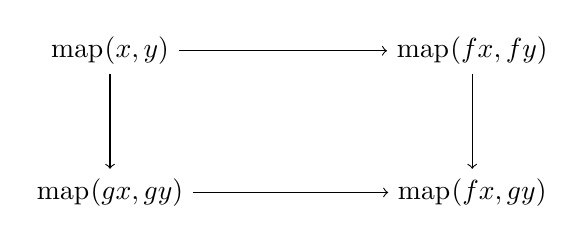
\begin{tikzpicture}
  \node (tl) at (0,0) {$\mathrm{map}_{\C}(x, y)$};
  \node (tr) at (4.6,0) {$\mathrm{map}_{\D}(fx, fy)$};
  \node (bl) at (0,-1.8) {$\mathrm{map}_{\D}(gx, gy)$};
  \node (br) at (4.6,-1.8) {$\mathrm{map}_{\D}(fx, gy)$};
  \draw[->] (tl) -- (tr);
  \draw[->] (tl) -- (bl);
  \draw[->] (tr) -- (br);
  \draw[->] (bl) -- (br);
\end{tikzpicture}
\end{center}
在\trHomotopy{}意义下交换。如果 $\tau$ 是一个\trNaturalEquivalence{}，那么下面的
水平映射与右边的竖直映射都是\trEquivalence{}。特别地，如果 $\D = \C$ 且
$g = \mathrm{id}_{\C}$，我们发现：如果 $f$ 等价于 $\mathrm{id}_{\C}$，那么映射
\[
\mathrm{map}_{\C}(x, y) \longrightarrow \mathrm{map}_{\D}(fx, fy)
\]
是一个\trHomotopy{}等价。
\end{lemma}

\begin{proof}
回忆，由后复合诱导出一个\trFunctor{}%
$\mathrm{Fun}(\C, \D) \longrightarrow \mathrm{Fun}(\C^{\Delta^1}, \D^{\Delta^1})$。
于是给定的\trNaturalTransformation{} $\tau$ 便诱导一个\trFunctor{}%
$\Delta^1 \longrightarrow \mathrm{Fun}(\C^{\Delta^1}, \D^{\Delta^1})$，后者
（由\trAdjunction{}）是一个\trFunctor{}%
\[
\C^{\Delta^1} \longrightarrow \D^{\Delta^1 \times \Delta^1}.
\]
展开这个构造，我们发现这个\trFunctor{}把一个\trMorphism{} $x \to y$ 送到图表
\begin{center}
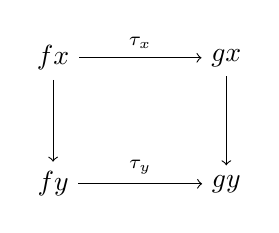
\begin{tikzpicture}
  \node (fx) at (0,0) {$fx$};
  \node (gx) at (2.2,0) {$gx$};
  \node (fy) at (0,-1.6) {$fy$};
  \node (gy) at (2.2,-1.6) {$gy$};
  \draw[->] (fx) -- node[above] {\scriptsize $\tau_x$} (gx);
  \draw[->] (fx) -- (fy);
  \draw[->] (gx) -- (gy);
  \draw[->] (fy) -- node[above] {\scriptsize $\tau_y$} (gy);
\end{tikzpicture}
\end{center}
因此，我们得到图表
\begin{center}
\begin{tikzpicture}
  \node (a) at (0,0) {$\C^{\Delta^1}$};
  \node (b) at (3.6,0) {$\D^{\Delta^1 \times \Delta^1}$};
  \node (c) at (8.2,0) {$\D^{\Delta^1} \times_{\D} \D^{\Delta^1}$};
  \node (d) at (3.6,-1.9) {$\D^{\Delta^1} \times_{\D} \D^{\Delta^1}$};
  \node (e) at (8.2,-1.9) {$\D^{\Delta^1}$};
  \draw[->] (a) -- (b);
  \draw[->] (b) -- (c);
  \draw[->] (b) -- (d);
  \draw[->] (c) -- (e);
  \draw[->] (b) -- (e);
  \draw[->] (d) -- (e);
\end{tikzpicture}
\end{center}
其中，从 $\D^{\Delta^1 \times \Delta^1}$ 出发的那个水平\trFunctor{}由沿映射
$\Lambda^2_1 \to \Delta^1 \times \Delta^1$ 的限制给出，这个映射挑出正方形的
一个角；而竖直\trFunctor{}则由沿映射 $\Lambda^2_1 \to \Delta^1 \times \Delta^1$
的限制给出，这个映射挑出另一个角。对角映射由沿包含
$\Delta^1 \to \Delta^1 \times \Delta^1$ 的限制给出，后者把 $0$ 送到 $(0, 0)$、
把 $1$ 送到 $(1, 1)$。其余两个\trFunctor{}由复合给出。两个三角形都在%
\trNaturalEquivalence{}的意义下交换（这就需要选取平凡纤维化
$\D^{\Delta^2} \to \D^{\Lambda^2_1}$ 的一个截面）。

现在我们固定 $\C$ 的两个\trObject{} $x$ 与 $y$，并考虑包含
$\mathrm{map}_{\C}(x, y) \longrightarrow \C^{\Delta^1}$。细察之下，我们发现图表
\begin{center}
\begin{tikzpicture}
  \node (tl) at (0,0) {$\mathrm{map}_{\C}(x, y)$};
  \node (tr) at (6.4,0) {$\{\tau_x\} \times \mathrm{map}_{\D}(gx, gy)$};
  \node (bl) at (0,-1.8) {$\C^{\Delta^1}$};
  \node (br) at (6.4,-1.8) {$\D^{\Delta^1} \times_{\D} \D^{\Delta^1}$};
  \draw[->, dashed] (tl) -- (tr);
  \draw[->] (tl) -- (bl);
  \draw[->] (tr) -- (br);
  \draw[->] (bl) -- (br);
\end{tikzpicture}
\end{center}
交换，也就是说，下面的复合如虚箭头所示那样分解。

对于把竖直映射限制到 $\mathrm{map}_{\C}(x, y)$ 上，同样的结论也成立，于是我们
最终得到图表
\begin{center}
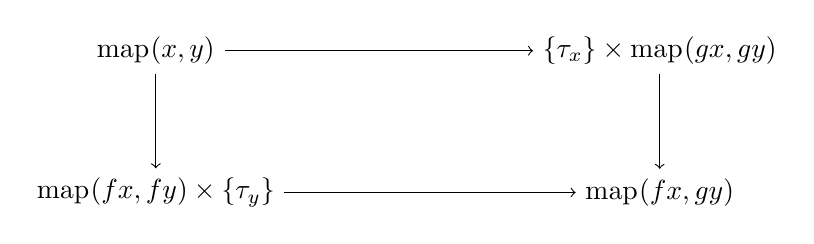
\begin{tikzpicture}
  \node (tl) at (0,0) {$\mathrm{map}_{\C}(x, y)$};
  \node (tr) at (6.4,0) {$\{\tau_x\} \times \mathrm{map}_{\D}(gx, gy)$};
  \node (bl) at (0,-1.8) {$\mathrm{map}_{\D}(fx, fy) \times \{\tau_y\}$};
  \node (br) at (6.4,-1.8) {$\mathrm{map}_{\D}(fx, gy)$};
  \draw[->] (tl) -- (tr);
  \draw[->] (tl) -- (bl);
  \draw[->] (tr) -- (br);
  \draw[->] (bl) -- (br);
\end{tikzpicture}
\end{center}
它在\trNaturalEquivalence{}的意义下交换，正如所需。
\end{proof}

\begin{proposition}\label{prop:joyal-equivalence-fully-faithful-essentially-surjective}
∞-\trCategories{}之间的\trJoyalEquivalence{}既是\trFullyFaithful{}又是%
\trEssentiallySurjective{}。
\end{proposition}

\begin{proof}
\trFunctor{} $h\C \to h\D$ 是一个\trEquivalence{}（见\cref{ex:joyal-equivalence-h}），从而是%
\trEssentiallySurjective{}。于是，依\cref{def:essentially-surjective}，
$\C \to \D$ 是\trEssentiallySurjective{}。为了证明全忠实性，选取 $f$ 的一个逆
$g$。那么，对于一对\trObject{} $x, y \in \C$，我们得到
\[
\mathrm{map}_{\C}(x, y) \longrightarrow \mathrm{map}_{\D}(fx, fy)
\longrightarrow \mathrm{map}_{\C}(gfx, gfy)
\longrightarrow \mathrm{map}_{\D}(fgfx, fgfy).
\]
由于\trFunctor{} $gf$ 自然等价于 $\mathrm{id}_{\C}$，而\trFunctor{} $fg$ 自然等价于
$\mathrm{id}_{\D}$，我们看到：前两个映射的复合与后两个映射的复合都是%
\trEquivalence{}。这蕴含中间的映射自身是一个\trEquivalence{}（它同时拥有左逆与
右逆），从而第一个映射也是一个\trEquivalence{}（作为某个\trEquivalence{}的右逆）。
\end{proof}

\begin{remark}\label{rem:enriched-alternative}
或者，人们可以如下论证：由\cref{ex:composition-enriched-hkan}，我们发现每个∞-\trCategory{}都给出一个在%
\trKanComplex{}的\trHomotopyCategory{} $h(\mathrm{Kan})$ 上充实的\trCategory{}，因为合成在%
\trHomotopy{}意义下是良定义的。利用这个结果，我们发现：\trFunctor{}%
$f\colon \C \to \D$ 是一个\trJoyalEquivalence{}，当且仅当诱导的
$h(\mathrm{Kan})$-充实\trCategories{}之间的\trFunctor{}是一个\trEquivalence{}。
同样地，它既\trFullyFaithful{}又\trEssentiallySurjective{}，当且仅当诱导的
$h(\mathrm{Kan})$-充实\trCategories{}之间的\trFunctor{}是\trFullyFaithful{}。
由这一分析，我们推出：如果 $f$ 自然等价于 $g$，那么 $f$ 是\trFullyFaithful{}%
当且仅当 $g$ 是\trFullyFaithful{}。在上面的论证中，我们可以把这个结果应用于
$gf$；后者与 $\mathrm{id}_{\C}$ 等价，从而其自身必是\trFullyFaithful{}，于是
所需的映射事实上是一个\trHomotopy{}等价。
\end{remark}

为了便于今后的引用，我们记录下面两个引理。

\begin{lemma}\label{lem:full-subcategory-fully-faithful}
一个满子范畴的包含 $\C_0 \subseteq \C$ 是一个\trFullyFaithful{}\trFunctor{}。
\end{lemma}

\begin{proof}
我们首先观察到：对每个∞-\trCategory{} $\D$，∞-\trCategory{}%
$\mathrm{Fun}(\D, \C_0)$ 是 $\mathrm{Fun}(\D, \C)$ 的由那些经过
$\C_0 \subseteq \C$ 分解的\trFunctor{}构成的满子范畴（见\cref{ex:functor-category-full-sub}）。利用这个
结果，我们可以推出图表
\begin{center}
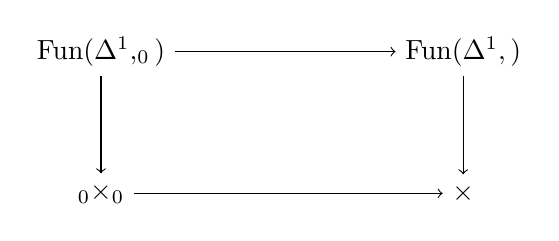
\begin{tikzpicture}
  \node (tl) at (0,0) {$\mathrm{Fun}(\Delta^1, \C_0)$};
  \node (tr) at (4.6,0) {$\mathrm{Fun}(\Delta^1, \C)$};
  \node (bl) at (0,-1.8) {$\C_0 \times \C_0$};
  \node (br) at (4.6,-1.8) {$\C \times \C$};
  \draw[->] (tl) -- (tr);
  \draw[->] (tl) -- (bl);
  \draw[->] (tr) -- (br);
  \draw[->] (bl) -- (br);
\end{tikzpicture}
\end{center}
是一个\trPullback{}。通过过渡到 $\C_0 \times \C_0$ 中\trObject{} $(x, y)$ 之上
的\trFibre{}，这就蕴含了本引理。
\end{proof}

\begin{lemma}\label{lem:map-simeq-inclusion}
设 $\C$ 是一个∞-\trCategory{}，并设 $x, y$ 是 $\C$ 的\trObject{}。那么映射
\[
\mathrm{map}_{\C^{\simeq}}(x, y) \longrightarrow \mathrm{map}_{\C}(x, y)
\]
是那些点皆为 $\C$ 中\trEquivalence{}的道路分支的包含。
\end{lemma}

\begin{proof}
我们将证明：任何映射 $\Delta^n \to \mathrm{map}_{\C}(x, y)$ 都提升为指向
$\mathrm{map}_{\C^{\simeq}}(x, y)$ 的映射，如果对每个 $i \in \Delta^n$，相应的从
$x$ 到 $y$ 的\trMorphism{}是一个\trEquivalence{}。为此，我们考虑一个映射
$\Delta^n \to \mathrm{map}_{\C}(x, y)$，使得对每个 $i \in \Delta^n$，其伴随映射的
限制
\[
\{i\} \times \Delta^1 \longrightarrow \Delta^n \times \Delta^1 \longrightarrow \C
\]
表示 $\C$ 中的一个\trEquivalence{}。于是我们观察到：对所有 $\epsilon = 0, 1$，
\[
\Delta^n \times \{\epsilon\} \longrightarrow \Delta^n \times \Delta^1 \longrightarrow \C
\]
是常值的（取值为 $x$ 或 $y$），从而也表示 $\C$ 的一个\trEquivalence{}。由于
$\Delta^n \times \Delta^1$ 中的所有\trMorphism{}都是前述形态的\trMorphism{}的
复合，我们可以推出：映射
\[
\Delta^n \times \Delta^1 \longrightarrow \C
\]
经过 $\C^{\simeq}$ 分解，这就证明了断言。
\end{proof}

接下来，我们的目标是证明\cref{prop:joyal-equivalence-fully-faithful-essentially-surjective} 的逆命题：一个既\trFullyFaithful{}又\trEssentiallySurjective{}%
\trFunctor{}是一个\trJoyalEquivalence{}。为此，我们需要下面几个准备性的陈述。

\begin{lemma}\label{lem:core-fully-faithful-essentially-surjective}
如果 $f\colon \C \to \D$ 既\trFullyFaithful{}又\trEssentiallySurjective{}，那么
$f^{\simeq}\colon \C^{\simeq} \to \D^{\simeq}$ 也是如此。
\end{lemma}

\begin{proof}
本质满性是显然的，因为 $\C^{\simeq}$ 与 $\C$ 拥有相同的\trObject{}。全忠实性也
不成问题：由于映射
$\mathrm{map}_{\C^{\simeq}}(x, y) \subseteq \mathrm{map}_{\C}(x, y)$ 是一些道路
分支的汇集（见\cref{lem:map-simeq-inclusion}），只需在 $\C$ 与 $\D$ 为%
\trOrdinaryCategory{}的情形下（借助\trHomotopyCategory{}）知道本引理的结论即可，而这是一个
显式且容易的验证。
\end{proof}

我们将用到\trKanFibration{}的如下基本性质，参见例如
\cite[Lemma 7.3]{GJ09}。

\begin{lemma}\label{lem:kan-fibration-long-exact-sequence}
设 $f\colon X \to Y$ 是\trKanComplex{}之间的一个\trKanFibration{}。设 $x$ 是 $X$
中的一个点，并设 $F$ 是 $f$ 在点 $y = f(x)$ 之上的\trFibre{}。那么存在一个长正合列
\[
\begin{aligned}
\dotsb \longrightarrow \pi_{n+1}(Y, y) \xrightarrow{\ \partial\ }
\pi_n(F, x) \longrightarrow \pi_n(X, x)\; &\xrightarrow{\ f_*\ }\\
\pi_n(Y, y) \xrightarrow{\ \partial\ } \dotsb
\longrightarrow \pi_0(X) \longrightarrow \pi_0(Y),
\end{aligned}
\]
它关于纤维化之间的\trMorphism{}是自然的；当 $n \ge 1$ 时它是群的正合列，而当
$n = 0$ 时它是带基点集合的正合列。
\end{lemma}

此外，我们将需要\trWhitehead{}（Whitehead）定理：

\begin{proposition}\label{prop:whitehead}
设 $f\colon X \to Y$ 是\trKanComplex{}之间的一个在道路分支上诱导双射的映射。
那么 $f$ 是一个\trHomotopy{}等价，当且仅当对所有点 $x \in X$ 与所有 $n \ge 1$，
诱导映射
\[
f_*\colon \pi_n(X, x) \longrightarrow \pi_n(Y, y)
\]
是一个双射。
\end{proposition}

至于证明，可由例如 \cite[I.11.3 \& II.1.10]{GJ09} 拼合而得。

\begin{corollary}\label{cor:kan-complex-ffes-homotopy-equivalence}
\trKanComplex{}之间一个既\trFullyFaithful{}又\trEssentiallySurjective{}%
\trFunctor{} $f\colon X \to Y$ 是一个\trHomotopy{}等价。
\end{corollary}

\begin{proof}
由于该\trFunctor{}诱导\trHomotopyCategory{}之间的一个\trEquivalence{}，我们发现映射 $f$
诱导一个双射 $\pi_0(X) \to \pi_0(Y)$。我们希望证明：对所有 $x \in X$ 与所有
$n \ge 1$，诱导映射
\[
\pi_n(X, x) \longrightarrow \pi_n(Y, y)
\]
也是一个双射，其中 $y = f(x)$。为此，我们考虑图表
\begin{center}
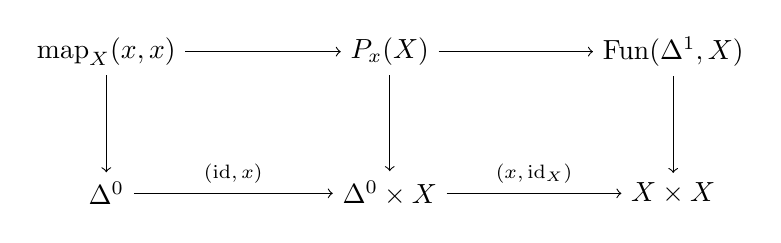
\begin{tikzpicture}
  \node (tl) at (0,0) {$\mathrm{map}_X(x, x)$};
  \node (tm) at (3.6,0) {$P_x(X)$};
  \node (tr) at (7.2,0) {$\mathrm{Fun}(\Delta^1, X)$};
  \node (bl) at (0,-1.8) {$\Delta^0$};
  \node (bm) at (3.6,-1.8) {$\Delta^0 \times X$};
  \node (br) at (7.2,-1.8) {$X \times X$};
  \draw[->] (tl) -- (tm);
  \draw[->] (tm) -- (tr);
  \draw[->] (tl) -- (bl);
  \draw[->] (tm) -- (bm);
  \draw[->] (tr) -- (br);
  \draw[->] (bl) -- node[above] {\scriptsize $(\mathrm{id}, x)$} (bm);
  \draw[->] (bm) -- node[above] {\scriptsize $(x, \mathrm{id}_X)$} (br);
\end{tikzpicture}
\end{center}
由于最右边的竖直映射是\trKanComplex{}之间的一个\trIsofibration{}，它是一个%
\trKanFibration{}。于是，中间的竖直映射也是一个\trKanFibration{}。这个构造关于
$X$ 显然是自然的，因此我们得到一个 Kan \trFibreSequence{}的图表
\begin{center}
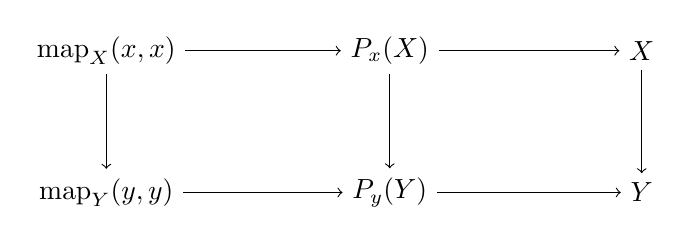
\begin{tikzpicture}
  \node (tl) at (0,0) {$\mathrm{map}_X(x, x)$};
  \node (tm) at (3.6,0) {$P_x(X)$};
  \node (tr) at (6.8,0) {$X$};
  \node (bl) at (0,-1.8) {$\mathrm{map}_Y(y, y)$};
  \node (bm) at (3.6,-1.8) {$P_y(Y)$};
  \node (br) at (6.8,-1.8) {$Y$};
  \draw[->] (tl) -- (tm);
  \draw[->] (tm) -- (tr);
  \draw[->] (tl) -- (bl);
  \draw[->] (tm) -- (bm);
  \draw[->] (tr) -- (br);
  \draw[->] (bl) -- (bm);
  \draw[->] (bm) -- (br);
\end{tikzpicture}
\end{center}
其中竖直映射由映射 $f\colon X \to Y$ 诱导。我们现在证明 $P_x(X)$ 可缩。为此，
注意它也出现在\trPullback{}图表
\begin{center}
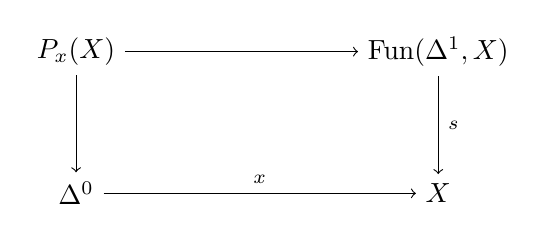
\begin{tikzpicture}
  \node (tl) at (0,0) {$P_x(X)$};
  \node (tr) at (4.6,0) {$\mathrm{Fun}(\Delta^1, X)$};
  \node (bl) at (0,-1.8) {$\Delta^0$};
  \node (br) at (4.6,-1.8) {$X$};
  \draw[->] (tl) -- (tr);
  \draw[->] (tl) -- (bl);
  \draw[->] (tr) -- node[right] {\scriptsize $s$} (br);
  \draw[->] (bl) -- node[above] {\scriptsize $x$} (br);
\end{tikzpicture}
\end{center}
之中，其中 $t$ 表示目标映射，即沿 $\{0\} \to \Delta^1$ 取限制所得到的映射。
\footnote{译注：原书图中该箭头标作 $s$，而正文却称 $t$，两处不一致，兹照录
原文。——译者注}由于映射 $\{0\} \to \Delta^1$ 是\trAnodyne{}的，而 $X$ 是一个%
\trKanComplex{}，所得到的映射 $\mathrm{Fun}(\Delta^1, X) \to X$ 是一个%
\trTrivialFibration{}，从而映射 $P_x(X) \to \Delta^0$ 也是一个\trTrivialFibration{}。
这蕴含 $P_x(X)$ 的确可缩。

于是我们得到：对所有 $n \ge 1$，存在交换图表
\begin{center}
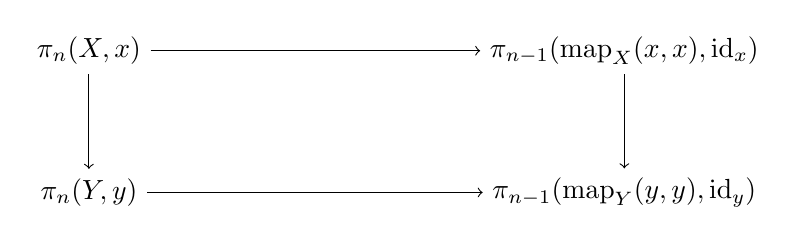
\begin{tikzpicture}
  \node (tl) at (0,0) {$\pi_n(X, x)$};
  \node (tr) at (6.8,0) {$\pi_{n-1}(\mathrm{map}_X(x, x), \mathrm{id}_x)$};
  \node (bl) at (0,-1.8) {$\pi_n(Y, y)$};
  \node (br) at (6.8,-1.8) {$\pi_{n-1}(\mathrm{map}_Y(y, y), \mathrm{id}_y)$};
  \draw[->] (tl) -- (tr);
  \draw[->] (tl) -- (bl);
  \draw[->] (tr) -- (br);
  \draw[->] (bl) -- (br);
\end{tikzpicture}
\end{center}
其中水平映射是同构，所据是\cref{lem:kan-fibration-long-exact-sequence} 的长正合列
以及 $P_x(X)$ 与 $P_y(Y)$ 的可缩性。由于 $f$ 是\trFullyFaithful{}，映射
$\mathrm{map}_X(x, x) \to \mathrm{map}_Y(y, y)$ 是一个\trHomotopy{}等价，从而在
所有同伦群上诱导双射。由此得出，左边的竖直映射也是一个同构。
\end{proof}

\begin{corollary}\label{cor:ffes-groupoid-core}
∞-\trCategories{}之间一个既\trFullyFaithful{}又\trEssentiallySurjective{}%
\trFunctor{}在\trGroupoid{}核上诱导一个\trHomotopy{}等价。
\end{corollary}

\begin{proof}
由\cref{lem:core-fully-faithful-essentially-surjective}，在\trGroupoid{}核上诱导的%
\trFunctor{}仍是\trEssentiallySurjective{}且\trFullyFaithful{}，于是
\cref{cor:kan-complex-ffes-homotopy-equivalence} 适用。
\end{proof}

为了\cref{lem:pullback-weak-equivalence}，我们将需要\emph{\trReedy{}（Reedy）引理}，
即下述陈述。事实上，它在任何%
\trModelCategory{}中都成立。至于一般\trModelCategory{}中的证明，我们参考
\cite[Prop.~13.1.2]{Hir03}。

\begin{lemma}\label{lem:reedy}
考虑\trPullback{}图表
\begin{center}
\begin{tikzpicture}
  \node (tl) at (0,0) {$C \times_A B$};
  \node (tr) at (3.2,0) {$B$};
  \node (bl) at (0,-1.8) {$C$};
  \node (br) at (3.2,-1.8) {$A$};
  \draw[->] (tl) -- (tr);
  \draw[->] (tl) -- (bl);
  \draw[->] (tr) -- node[right] {\scriptsize $p$} (br);
  \draw[->] (bl) -- node[above] {$\simeq$} node[below] {\scriptsize $f$} (br);
\end{tikzpicture}
\end{center}
其中 $p$ 是一个纤维化，而 $f$ 是\trFibrantObject{}之间的一个\trWeakEquivalence{}。那么
映射 $C \times_A B \to B$ 也是一个\trWeakEquivalence{}。
\end{lemma}

\begin{remark}\label{rem:reedy-simplicial}
对于\trSimplicialSets{}，让我们假设手头已有\trKanFibration{}的同伦群长正合列可供
使用。在这种情形下，通过追图（diagram chase）——利用竖直纤维化的长正合列——我们
容易发现：诱导映射
\[
\pi_i(C \times_A B, x) \longrightarrow \pi_i(B, x')
\]
对每个基点 $x \in C \times_A B$ 与每个 $i \ge 1$ 都是双射。为了对我们感兴趣的情形
证明\trReedy{}引理，于是只剩下要看映射 $C \times_A B \to B$ 在道路分支上诱导一个双射。
为此，这里的论证与\cref{lem:kan-fibration-surjection-pi0} 的证明中所用的论证
非常相似。
让我们首先证明这个映射的满性：选取 $B$ 中表示类 $[b] \in \pi_0(B)$ 的一个点
$b$，并考虑 $A$ 中的点 $p(b)$。由于 $C \to A$ 在道路分支上诱导一个双射，我们可以
找到一个点 $c \in C$ 与一条把 $f(c)$ 连到 $p(b)$ 的道路 $\Delta^1 \to A$。如
\cref{lem:kan-fibration-surjection-pi0} 中那样，这给出一个提升问题
\begin{center}
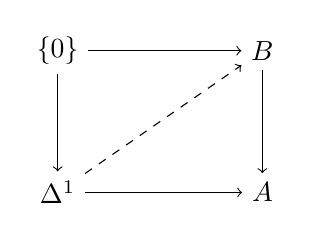
\begin{tikzpicture}
  \node (v) at (0,0) {$\{0\}$};
  \node (c) at (2.6,0) {$B$};
  \node (d1) at (0,-1.8) {$\Delta^1$};
  \node (d) at (2.6,-1.8) {$A$};
  \draw[->] (v) -- (c);
  \draw[->] (v) -- (d1);
  \draw[->] (c) -- (d);
  \draw[->] (d1) -- (d);
  \draw[->, dashed] (d1) -- (c);
\end{tikzpicture}
\end{center}
由于 $p$ 是\trKanFibration{}，它可以求解。于是我们发现：存在 $B$ 中的一个
$b'$，使得 $p(b') = f(c)$，并且在 $\pi_0(B)$ 中 $[b'] = [b]$。因此，二元组
$(c, b')$ 确定 $\pi_0(C \times_A B)$ 的一个元素，后者在 $\pi_0(B)$ 中被送到
$[b]$。这表明映射 $\pi_0(C \times_A B) \to \pi_0(B)$ 的确是满的。

为了证明单性，考虑 $C \times_A B$ 的两个点 $(c, b)$ 与 $(c', b')$，并假设
存在一条道路 $\alpha\colon \Delta^1 \to B$，它在 $B$ 中连接 $b$ 与 $b'$。那么
$p(\alpha)\colon \Delta^1 \to A$ 连接 $p(b) = f(c)$ 与 $p(b') = f(c')$。由于
映射 $f$ 是一个\trHomotopy{}等价，存在一条道路 $\beta\colon \Delta^1 \to C$，
使得 $f_*(\beta)$ 等价于 $p_*(\alpha)$。更精确地，我们可以找到一个%
\trTwoCell{} $\sigma\colon \Delta^2 \to A$，使得
\begin{enumerate}[label=(\arabic*)]
  \item $\sigma|_{\Delta^{\{0,1\}}} = f_*(\beta)$，
  \item $\sigma|_{\Delta^{\{1,2\}}} = \mathrm{id}_{f(c')}$，并且
  \item $\sigma|_{\Delta^{\{0,2\}}} = p_*(\alpha)$。
\end{enumerate}
由于我们可以沿 $p$ 同时提升 $p_*(\alpha)$ 与 $\mathrm{id}_{f(c')}$，与%
\cref{lem:kan-fibration-surjection-pi0} 中类似，我们得到图表
\begin{center}
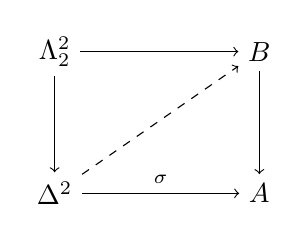
\begin{tikzpicture}
  \node (l) at (0,0) {$\Lambda^2_2$};
  \node (r) at (2.6,0) {$B$};
  \node (dl) at (0,-1.8) {$\Delta^2$};
  \node (dr) at (2.6,-1.8) {$A$};
  \draw[->] (l) -- (r);
  \draw[->] (l) -- (dl);
  \draw[->] (r) -- (dr);
  \draw[->] (dl) -- node[above] {\scriptsize $\sigma$} (dr);
  \draw[->, dashed] (dl) -- (r);
\end{tikzpicture}
\end{center}
而由于 $p$ 是\trKanFibration{}，该图表容有如图所示的虚箭头。由此得出：存在一条
连接 $b$ 与 $b'$ 的道路 $\gamma\colon \Delta^1 \to B$，使得
$p_*(\gamma) = f_*(\beta)$。因此，$\gamma$ 与 $\beta$ 拼合成一个映射
$\Delta^1 \to C \times_A B$，它连接 $(c, b)$ 与 $(c', b')$。这表明所论映射是
单的。
\end{remark}

\begin{lemma}\label{lem:pullback-weak-equivalence}
考虑\trKanComplex{}的一张图表
\begin{center}
\begin{tikzpicture}
  \node (c) at (0,0) {$C$};
  \node (a) at (3.2,0) {$A$};
  \node (b) at (6.4,0) {$B$};
  \node (c2) at (0,-2) {$C'$};
  \node (a2) at (3.2,-2) {$A'$};
  \node (b2) at (6.4,-2) {$B'$};
  \draw[->>] (c) -- (a);
  \draw[<-] (a) -- (b);
  \draw[->>] (c2) -- (a2);
  \draw[<-] (a2) -- (b2);
  \draw[->] (c) -- node[right] {$\simeq$} (c2);
  \draw[->] (a) -- node[right] {$\simeq$} (a2);
  \draw[->] (b) -- node[right] {$\simeq$} (b2);
\end{tikzpicture}
\end{center}
其中竖直映射都是\trWeakEquivalence{}，而左边的水平映射都是\trKanFibration{}。
那么\trPullback{}上诱导的映射
\[
C \times_A B \longrightarrow C' \times_{A'} B'
\]
仍是\trWeakEquivalence{}。
\end{lemma}

\begin{proof}
我们首先把眼前的情形化归为映射 $B \to A$ 与 $B' \to A'$ 也是纤维化的情形：由%
\trSmallObjectArgument{}，通过对映射 $B \to A$ 作函子式分解——一个%
\trWeakEquivalence{}后接一个纤维化（在我们的情形是一个\trAnodyneMap{}后接一个%
\trKanFibration{}）——我们得到交换图表
\begin{center}
\begin{tikzpicture}
  \node (a) at (0,0) {$A$};
  \node (d) at (3.2,0) {$D$};
  \node (b) at (6.4,0) {$B$};
  \node (a2) at (0,-2) {$A'$};
  \node (d2) at (3.2,-2) {$D'$};
  \node (b2) at (6.4,-2) {$B'$};
  \draw[->>] (d) -- (a);
  \draw[<-] (d) -- node[below] {$\simeq$} (b);
  \draw[->>] (d2) -- (a2);
  \draw[<-] (d2) -- node[below] {$\simeq$} (b2);
  \draw[->] (a) -- (a2);
  \draw[->] (d) -- (d2);
  \draw[->] (b) -- (b2);
\end{tikzpicture}
\end{center}
由此可知 $D$ 与 $D'$ 都是纤维性的，并且我们得到交换图表
\begin{center}
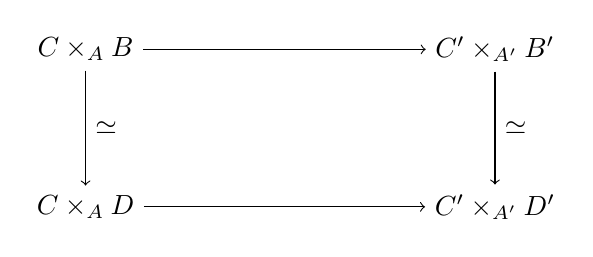
\begin{tikzpicture}
  \node (tl) at (0,0) {$C \times_A B$};
  \node (tr) at (5.2,0) {$C' \times_{A'} B'$};
  \node (bl) at (0,-2) {$C \times_A D$};
  \node (br) at (5.2,-2) {$C' \times_{A'} D'$};
  \draw[->] (tl) -- (tr);
  \draw[->] (tl) -- node[right] {$\simeq$} (bl);
  \draw[->] (tr) -- node[right] {$\simeq$} (br);
  \draw[->] (bl) -- (br);
\end{tikzpicture}
\end{center}
我们希望证明其中上面的水平映射是\trEquivalence{}。我们断言两个竖直映射都是%
\trEquivalence{}：例如，左边的竖直映射出现在\trPullback{}图表
\begin{center}
\begin{tikzpicture}
  \node (tl) at (0,0) {$C \times_A B$};
  \node (tm) at (4.0,0) {$C \times_A D$};
  \node (tr) at (8.0,0) {$C$};
  \node (bl) at (0,-2) {$B$};
  \node (bm) at (4.0,-2) {$D$};
  \node (br) at (8.0,-2) {$A$};
  \draw[->] (tl) -- (tm);
  \draw[->] (tm) -- (tr);
  \draw[->] (tl) -- (bl);
  \draw[->] (tm) -- (bm);
  \draw[->] (tr) -- (br);
  \draw[->] (bl) -- node[above] {$\simeq$} (bm);
  \draw[->] (bm) -- (br);
\end{tikzpicture}
\end{center}
之中，于是\trReedy{}引理蕴含上面的水平映射是\trEquivalence{}。（映射
$C \times_A D \to D$ 是一个纤维化，因为它由 $C \to A$ 拉回而得，而后者由假设是
一个纤维化。）对右边竖直映射的论证是类似的。

于是我们可以假定：在引理的陈述中，所有水平映射实际上都是纤维化。注意，所论
映射分解为复合
\[
C \times_A B \longrightarrow (C' \times_{A'} A) \times_A B
= C' \times_{A'} B \longrightarrow C' \times_{A'} B'.
\]

现在我们可以三次使用\trReedy{}引理：
\begin{enumerate}[label=(\arabic*)]
  \item 映射 $C \to C' \times_{A'} A$ 是\trEquivalence{}：由\trReedy{}引理，映射
  $C' \times_{A'} A \to C'$ 是\trWeakEquivalence{}，因为它出现在\trPullback{}%
  \begin{center}
  \begin{tikzpicture}
    \node (tl) at (0,0) {$C' \times_{A'} A$};
    \node (tr) at (3.2,0) {$C'$};
    \node (bl) at (0,-1.8) {$A$};
    \node (br) at (3.2,-1.8) {$A'$};
    \draw[->] (tl) -- (tr);
    \draw[->] (tl) -- (bl);
    \draw[->] (tr) -- (br);
    \draw[->] (bl) -- node[above] {$\simeq$} (br);
  \end{tikzpicture}
  \end{center}
  之中。于是，在复合
  \[
  C \longrightarrow C' \times_{A'} A \longrightarrow C',
  \]
  中，第二个映射与复合都是\trEquivalence{}。然后，诸\trEquivalence{}的%
  \trThreeForTwoProperty{}便确认了这一断言。
  \item 映射 $C \times_A B \to (C' \times_{A'} A) \times_A B$ 是一个%
  \trEquivalence{}：它出现在\trPullback{}方形
  \begin{center}
  \begin{tikzpicture}
    \node (tl) at (0,0) {$C \times_A B$};
    \node (tm) at (5.2,0) {$(C' \times_{A'} A) \times_A B$};
    \node (tr) at (9.6,0) {$B$};
    \node (bl) at (0,-1.8) {$C$};
    \node (bm) at (5.2,-1.8) {$C' \times_{A'} A$};
    \node (br) at (9.6,-1.8) {$A$};
    \draw[->] (tl) -- (tm);
    \draw[->] (tm) -- (tr);
    \draw[->] (tl) -- (bl);
    \draw[->] (tm) -- (bm);
    \draw[->] (tr) -- (br);
    \draw[->] (bl) -- (bm);
    \draw[->] (bm) -- (br);
  \end{tikzpicture}
  \end{center}
  之中，其中中间的竖直映射是纤维化，因为它由映射 $B \to A$ 拉回而得，后者现在由
  假设是纤维化。下面的水平映射由前一步是\trEquivalence{}，于是断言再次由%
  \trReedy{}引理得出。
  \item 映射 $C' \times_{A'} B \to C' \times_{A'} B'$ 是一个\trEquivalence{}：
  它出现在\trPullback{}方形
  \begin{center}
  \begin{tikzpicture}
    \node (tl) at (0,0) {$C' \times_{A'} B$};
    \node (tm) at (4.4,0) {$C' \times_{A'} B'$};
    \node (tr) at (8.0,0) {$C'$};
    \node (bl) at (0,-1.8) {$B$};
    \node (bm) at (4.4,-1.8) {$B'$};
    \node (br) at (8.0,-1.8) {$A'$};
    \draw[->] (tl) -- (tm);
    \draw[->] (tm) -- (tr);
    \draw[->] (tl) -- (bl);
    \draw[->] (tm) -- (bm);
    \draw[->] (tr) -- (br);
    \draw[->] (bl) -- (bm);
    \draw[->] (bm) -- (br);
  \end{tikzpicture}
  \end{center}
  之中，其中右边的竖直映射是纤维化，因为它由 $C' \to A'$ 拉回而得，后者由假设也
  是纤维化。现在映射 $B \to B'$ 是\trEquivalence{}，于是我们再次用\trReedy{}引理
  得出结论。
\end{enumerate}
\end{proof}

我们将需要关于\trInverseLimit{}的一个类似的不变性陈述。下述结果的更一般版本
可以在 \cite[Theorem 19.9.1]{Hir03} 中找到。

\begin{lemma}\label{lem:inverse-limit-weak-equivalence}
考虑诸\trFunctor{} $\N^{\mathrm{op}} \to \mathrm{sSet}$ 之间的一个%
\trNaturalTransformation{}%
\begin{center}
\begin{tikzpicture}
  \node (d) at (0,0) {$\dotsb$};
  \node (x3) at (1.9,0) {$X_3$};
  \node (x2) at (4.3,0) {$X_2$};
  \node (x1) at (6.7,0) {$X_1$};
  \node (x0) at (9.1,0) {$X_0$};
  \node (d2) at (0,-2.2) {$\dotsb$};
  \node (y3) at (1.9,-2.2) {$Y_3$};
  \node (y2) at (4.3,-2.2) {$Y_2$};
  \node (y1) at (6.7,-2.2) {$Y_1$};
  \node (y0) at (9.1,-2.2) {$Y_0$};
  \draw[->>] (d) -- (x3);
  \draw[->>] (x3) -- (x2);
  \draw[->>] (x2) -- (x1);
  \draw[->>] (x1) -- (x0);
  \draw[->>] (d2) -- (y3);
  \draw[->>] (y3) -- (y2);
  \draw[->>] (y2) -- (y1);
  \draw[->>] (y1) -- (y0);
  \draw[->] (d) -- node[right] {$\simeq$} (d2);
  \draw[->] (x3) -- node[right] {$\simeq$} (y3);
  \draw[->] (x2) -- node[right] {$\simeq$} (y2);
  \draw[->] (x1) -- node[right] {$\simeq$} (y1);
  \draw[->] (x0) -- node[right] {$\simeq$} (y0);
\end{tikzpicture}
\end{center}
并假设所有水平映射都是纤维化，所有竖直映射都是\trWeakEquivalence{}，而且所有
对象都是\trKanComplex{}。那么诱导映射
\[
\lim_i X_i \longrightarrow \lim_i Y_i
\]
是一个\trEquivalence{}。
\end{lemma}

\begin{remark}\label{rem:inverse-limit-lim1}
同样，人们可以利用同伦群的长正合列来证明这个结果。也就是说，事实证明存在一个
正合列
\[
0 \longrightarrow \lim_i^1 \pi_{k+1}(X_i) \longrightarrow
\pi_k(\lim_i X_i) \longrightarrow \lim_i \pi_k(X_i) \longrightarrow 0
\]
于是，（小心地！）施以追图论证便表明：在我们的情形中，\trInverseLimit{}上诱导
的映射在所有同伦群上诱导一个双射。关于这样的证明，参见例如 \cite{Hir15}。
\end{remark}

\begin{lemma}\label{lem:fibre-wise-homotopy-equivalence}
考虑\trKanComplex{}的一个交换图表
\begin{center}
\begin{tikzpicture}
  \node (y1) at (0,0) {$Y'$};
  \node (y) at (2.8,0) {$Y$};
  \node (x1) at (0,-1.8) {$X'$};
  \node (x) at (2.8,-1.8) {$X$};
  \draw[->] (y1) -- node[above] {\scriptsize $f$} (y);
  \draw[->] (y1) -- node[right] {\scriptsize $p'$} (x1);
  \draw[->] (y) -- node[right] {\scriptsize $p$} (x);
  \draw[->] (x1) -- node[above] {\scriptsize $f'$} (x);
\end{tikzpicture}
\end{center}
其中映射 $p$ 是一个纤维化。假设 $f'$ 是一个\trHomotopy{}等价，并且对 $X'$ 的每个
$0$-\trSimplex{} $x'$，诸竖直\trFibre{}之间的诱导映射
$p'^{-1}(x') \to p^{-1}(x)$ 也是\trEquivalence{}。那么映射 $f$ 是一个%
\trHomotopy{}等价。
\end{lemma}

\begin{proof}
由\trReedy{}引理，我们可以不失一般性地假设 $f'$ 是恒等：我们可以径直把映射 $p$ 换成
典范映射 $X' \times_X Y \to X'$，同时保持诸\trFibre{}不变，并且知道映射
$X' \times_X Y \to Y$ 是一个\trEquivalence{}。

如果同伦群的长正合列可用，那么只需一个容易的追图便可看出：对 $Y'$ 中的每个点
$y'$ 与每个 $i \ge 1$，映射
\[
\pi_i(Y', y') \longrightarrow \pi_i(Y, y)
\]
是双射，其中 $y = f(y')$。于是剩下要证的只是：映射 $f$ 在道路分支上诱导一个
双射。

为了证明单性，假设给定 $Y'$ 中的两个点 $x, y$，它们在 $f$ 之下于 $Y$ 中的像由
一条道路 $\alpha\colon \Delta^1 \to Y$ 连通。换言之，我们有 $\alpha(0) = f(x)$
与 $\alpha(1) = f(y)$。由此得出，$p\alpha\colon \Delta^1 \to X$ 是一条介于
$p(f(x)) = p'(x)$ 与 $p(f(y)) = p'(y)$ 之间的道路。考虑提升问题
\begin{center}
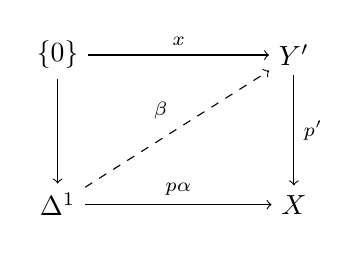
\begin{tikzpicture}
  \node (v) at (0,0) {$\{0\}$};
  \node (c) at (3.0,0) {$Y'$};
  \node (d1) at (0,-1.9) {$\Delta^1$};
  \node (d) at (3.0,-1.9) {$X$};
  \draw[->] (v) -- node[above] {\scriptsize $x$} (c);
  \draw[->] (v) -- (d1);
  \draw[->] (c) -- node[right] {\scriptsize $p'$} (d);
  \draw[->] (d1) -- node[above] {\scriptsize $p\alpha$} (d);
  \draw[->, dashed] (d1) -- node[above left] {\scriptsize $\beta$} (c);
\end{tikzpicture}
\end{center}
它可以求解，因为 $p'$ 是一个纤维化。\footnote{译注：原书此处标 $p$，依正文应为
$p'$。——译者注}于是我们有 $p'\beta = p\alpha$，而由于
$p' = pf$，我们得到 $pf\beta = p\alpha$。此外，我们有 $f\beta(0) = f(x) = \alpha(0)$。
于是我们得到提升问题
\begin{center}
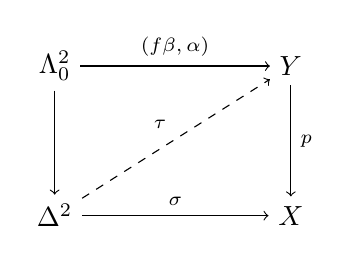
\begin{tikzpicture}
  \node (l) at (0,0) {$\Lambda^2_0$};
  \node (r) at (3.0,0) {$Y$};
  \node (dl) at (0,-1.9) {$\Delta^2$};
  \node (dr) at (3.0,-1.9) {$X$};
  \draw[->] (l) -- node[above] {\scriptsize $(f\beta, \alpha)$} (r);
  \draw[->] (l) -- (dl);
  \draw[->] (r) -- node[right] {\scriptsize $p$} (dr);
  \draw[->] (dl) -- node[above] {\scriptsize $\sigma$} (dr);
  \draw[->, dashed] (dl) -- node[above left] {\scriptsize $\tau$} (r);
\end{tikzpicture}
\end{center}
其中 $\sigma$ 是道路 $p\alpha$ 的一个退化。这个提升问题可以求解，因为 $p$ 是一个%
\trKanFibration{}。通过把虚箭头 $\tau$ 限制到 $\Delta^{\{1,2\}}$ 上，我们得到
一条从 $f(y)$ 到 $f(\beta(1))$ 的道路，它在 $p$ 之下被送到 $p'(y)$ 处的常值道路。
换言之，$\tau|_{\Delta^{\{1,2\}}}$ 是 $p^{-1}(p'(y))$ 中的一条道路。由于 $f$
限制为这个纤维上的一个\trHomotopy{}等价，在 $p'^{-1}(p'(y))$ 内部，$y$ 与
$\beta(1)$ 之间也存在一条道路。由于 $\beta(1)$（经由 $\beta$）与 $x$ 是连通的，
我们发现 $x$ 与 $y$ 由 $Y'$ 中的一条道路连通。

为了证明满性，考虑 $Y$ 的一个点 $y$，并令 $x = p(y)$。由定义，$y$ 落在 $p$ 在
$x$ 之上的\trFibre{} $F_x$ 中。这表明 $F_x$ 非空。由假设，映射 $f$ 限制为一个%
\trHomotopy{}等价 $F_x \simeq F'_x$，其中后者表示 $p'$ 在 $x$ 之上的%
\trFibre{}。\footnote{译注：原书印作「映射 $f'$ 限制为……」，但依本引理的假设
（$f'$ 已被简化为恒等），限制在诸\trFibre{}之间的应为 $f$，兹径改。——译者注}
选取 $F'_x$ 中的点 $y'$，使得 $[y']$ 在双射 $\pi_0(F'_x) \to \pi_0(F_x)$ 之下
对应于 $[y]$。\footnote{译注：原书印作「选取 $F'_x$ 中对应于 $[y]$ 的点
$y$」，但该点应记作 $y'$（下文明言 $\pi_0(Y') \to \pi_0(Y)$ 把 $[y']$ 送到
$[y]$），兹径改。——译者注}那么映射 $\pi_0(Y') \to \pi_0(Y)$ 把 $[y']$ 送到
$[y]$，也就是说，所论映射的确是满的。
\end{proof}

我们现在处于可以证明如下刻画的位置：\trJoyalEquivalence{}正是%
\trEssentiallySurjective{}且\trFullyFaithful{}\trFunctor{}。

\begin{theorem}\label{thm:ffes-joyal-equivalence}
∞-\trCategories{}之间一个既\trFullyFaithful{}又\trEssentiallySurjective{}%
\trFunctor{} $f\colon \C \to \D$ 是一个\trJoyalEquivalence{}。
\end{theorem}

\begin{proof}
我们将这样证明本定理：对任意\trSimplicialSet{} $X$，典范\trFunctor{}%
\[
f_*\colon (\C^X)^{\simeq} \longrightarrow (\D^X)^{\simeq}
\]
是一个\trHomotopy{}等价。一旦得证，便可取 $X = \D$，并通过取该\trHomotopy{}等价
的逆得到图表
\begin{center}
\begin{tikzpicture}
  \node (d0) at (0,0) {$\Delta^0$};
  \node (cd) at (4.2,0) {$(\C^{\D})^{\simeq}$};
  \node (d1) at (0,-1.8) {$\Delta^1$};
  \node (dd) at (4.2,-1.8) {$(\D^{\D})^{\simeq}$};
  \draw[->] (d0) -- node[above] {\scriptsize $g$} (cd);
  \draw[->] (d0) -- (d1);
  \draw[->] (cd) -- node[right] {\scriptsize $f_*$} (dd);
  \draw[->] (d1) -- node[above] {\scriptsize $h$} (dd);
\end{tikzpicture}
\end{center}
其中 $h$ 是从 $\mathrm{id}_{\D}$ 到 $fg$ 的一条道路，也就是说，$h$ 提供了 $fg$
与 $\mathrm{id}_{\D}$ 之间的一个\trNaturalEquivalence{}。为了看出 $gf$ 也自然
等价于 $\mathrm{id}_{\C}$，我们考虑\trHomotopy{}等价
\[
f_*\colon (\C^{\C})^{\simeq} \longrightarrow (\D^{\C})^{\simeq}
\]
并观察到 $\mathrm{id}_{\C}$ 被送到 $f$，而 $gf$ 被送到 $fgf$。但由于 $fg$ 与
$\mathrm{id}_{\D}$ 相连通，我们发现 $fgf$ 也经由一个\trNaturalEquivalence{}连通
到 $f$。由于上面的映射是\trHomotopy{}等价，这蕴含在 $\mathrm{id}_{\C}$ 与 $gf$
之间必定也存在一条道路，从而任何这样的道路都提供一个\trNaturalEquivalence{}%
$gf \simeq \mathrm{id}_{\C}$，于是 $f$ 与 $g$ 是互逆的\trFunctor{}。因此，$f$
是一个\trJoyalEquivalence{}。\footnote{译注：原书此两句印作「在
$\mathrm{id}_{\C}$ 与 $fg$ 之间必定也存在一条道路，从而任何这样的道路都提供一
个自然等价 $fg \simeq \mathrm{id}_{\C}$」；但 $fg\colon \D \to \D$ 并非
$(\C^{\C})^{\simeq}$ 中的对象，且此处所欲证者为 $gf$ 逆于 $f$，故两处均应为
$gf$，兹径改。——译者注}

我们现在来证明剩下的断言。为此，我们首先考虑 $X = \Delta^0$ 的情形。这等价于
如下陈述：$f$ 在\trGroupoid{}核上诱导一个\trHomotopy{}等价，这一点我们已在
\cref{cor:kan-complex-ffes-homotopy-equivalence} 中解决。接下来，我们处理
$X = \Delta^1$ 的情形。回忆源–目标映射 $\C^{\Delta^1} \to \C \times \C$ 是一个%
\trIsofibration{}，因此所得到的映射
\[
(\C^{\Delta^1})^{\simeq} \longrightarrow \C^{\simeq} \times \C^{\simeq}
\]
是一个\trKanFibration{}，并且它出现在交换方形
\begin{center}
\begin{tikzpicture}
  \node (tl) at (0,0) {$(\C^{\Delta^1})^{\simeq}$};
  \node (tr) at (4.6,0) {$\C^{\simeq} \times \C^{\simeq}$};
  \node (bl) at (0,-2) {$(\D^{\Delta^1})^{\simeq}$};
  \node (br) at (4.6,-2) {$\D^{\simeq} \times \D^{\simeq}$};
  \draw[->] (tl) -- (tr);
  \draw[->] (tl) -- (bl);
  \draw[->] (tr) -- node[right] {$\simeq$} (br);
  \draw[->] (bl) -- (br);
\end{tikzpicture}
\end{center}
之中，其中右边的竖直映射由前一步是\trHomotopy{}等价（再加上「%
\trJoyalEquivalence{}的乘积仍是\trJoyalEquivalence{}」这一观察）。依
\cref{lem:fibre-wise-homotopy-equivalence}，为了证明左边的竖直映射是%
\trHomotopy{}等价，只需证明：在点 $(x, y) \in \C^{\simeq} \times \C^{\simeq}$
之上的\trFibre{}上诱导的映射也是\trHomotopy{}等价。为此，我们观察到：图表
\begin{center}
\begin{tikzpicture}
  \node (tl) at (0,0) {$(\C^{\Delta^1})^{\simeq}$};
  \node (tr) at (3.8,0) {$\C^{\Delta^1}$};
  \node (bl) at (0,-1.9) {$\C^{\simeq} \times \C^{\simeq}$};
  \node (br) at (3.8,-1.9) {$\C \times \C$};
  \draw[->] (tl) -- (tr);
  \draw[->] (tl) -- (bl);
  \draw[->] (tr) -- (br);
  \draw[->] (bl) -- (br);
\end{tikzpicture}
\end{center}
是一个\trPullback{}，因为右边的竖直\trFunctor{}由
\cref{thm:bijective-on-vertices} 是\trConservative{}，于是我们可以援引
\cref{ex:conservative-pullback}。现在，上述方形中诸水平映射各自在点 $(x, y)$（相应地，在点
$(px, py)$）之上的\trFibre{}由相应的\trMappingSpace{}给出，这就建立了剩下的
断言。

接下来，我们处理 $X = I^n$ 的情形，即 $n$ 维\trSpine{}的情形。我们将通过对 $n$
的归纳证明：映射
\[
(\C^{I^n})^{\simeq} \longrightarrow (\D^{I^n})^{\simeq}
\]
是\trHomotopy{}等价。情形 $n = 1$ 已在前一步中完成。现在我们断言：存在如下%
\trPullback{}图表：
\begin{center}
\begin{tikzpicture}
  \node (tl) at (0,0) {$(\C^{I^n})^{\simeq}$};
  \node (tr) at (4.2,0) {$(\C^{I^{n-1}})^{\simeq}$};
  \node (bl) at (0,-1.9) {$(\C^{\Delta^1})^{\simeq}$};
  \node (br) at (4.2,-1.9) {$\C^{\simeq}$};
  \draw[->] (tl) -- (tr);
  \draw[->] (tl) -- (bl);
  \draw[->] (tr) -- (br);
  \draw[->] (bl) -- (br);
\end{tikzpicture}
\end{center}
由于 $I^n = I^{n-1} \amalg \Delta^1$，该图表在取\trGroupoid{}核之前是%
\trPullback{}，而且以 $\C$ 为目标的两个映射都是\trIsofibration{}（因为 $\C$
是一个∞-\trCategory{}，而映射 $\C \to \Delta^0$ 是\trIsofibration{}）。如
\cref{cor:equivalences-in-functor-pullback} 的证明中那样，于是只需观察到%
\trGroupoid{}核的\trPullback{}自身是一个∞-\trGroupoid{}。而事实正是如此，因为
右边的竖直映射是一个\trKanFibration{}（因为它在取\trGroupoid{}核之前是%
\trIsofibration{}）。映射 $\C \to \D$ 诱导从这个方形到相应方形（即通篇把
$\C$ 换成 $\D$ 而得的方形）的一个映射。在除左上角之外的所有位置上，这个映射由
归纳假设是\trHomotopy{}等价。因此，我们可以由\cref{lem:pullback-weak-equivalence}
得出断言。

接下来，我们处理 $X = \Delta^n$ 的情形。为此，我们考虑图表
\begin{center}
\begin{tikzpicture}
  \node (tl) at (0,0) {$(\C^{\Delta^n})^{\simeq}$};
  \node (tr) at (4.4,0) {$(\D^{\Delta^n})^{\simeq}$};
  \node (bl) at (0,-1.9) {$(\C^{I^n})^{\simeq}$};
  \node (br) at (4.4,-1.9) {$(\D^{I^n})^{\simeq}$};
  \draw[->] (tl) -- (tr);
  \draw[->] (tl) -- (bl);
  \draw[->] (tr) -- (br);
  \draw[->] (bl) -- (br);
\end{tikzpicture}
\end{center}
它由\trFunctor{} $\C \to \D$ 与包含 $I^n \to \Delta^n$ 诱导。由前一步，下面的
水平映射是\trHomotopy{}等价；而由\cref{thm:angle-fi-fibration}，诸竖直映射在取%
\trGroupoid{}核之前是\trTrivialFibration{}，从而在取\trGroupoid{}核之后仍是%
\trTrivialFibration{}。（限制到诸\trGroupoid{}核后所得的方形是一个\trPullback{}，
因为\trTrivialFibration{}是\trConservative{}。）由于\trTrivialFibration{}是%
\trHomotopy{}等价，我们由\trHomotopy{}等价的\trThreeForTwoProperty{}得出断言。

接下来我们处理一个任意但有限维的\trSimplicialSet{} $X$。我们按维数归纳地证明该
陈述。对 $0$ 维的 $X$，它再次由「\trJoyalEquivalence{}的乘积是%
\trJoyalEquivalence{}」这一事实得出。让我们证明归纳步骤，并假设 $X$ 是一个
$n$ 维\trSimplicialSet{}。考虑它的骨架推出
\begin{center}
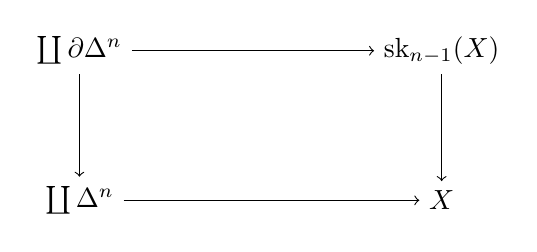
\begin{tikzpicture}
  \node (tl) at (0,0) {$\coprod \partial \Delta^n$};
  \node (tr) at (4.6,0) {$\mathrm{sk}_{n-1}(X)$};
  \node (bl) at (0,-1.9) {$\coprod \Delta^n$};
  \node (br) at (4.6,-1.9) {$X$};
  \draw[->] (tl) -- (tr);
  \draw[->] (tl) -- (bl);
  \draw[->] (tr) -- (br);
  \draw[->] (bl) -- (br);
\end{tikzpicture}
\end{center}
它诱导一个\trPullback{}方形
\begin{center}
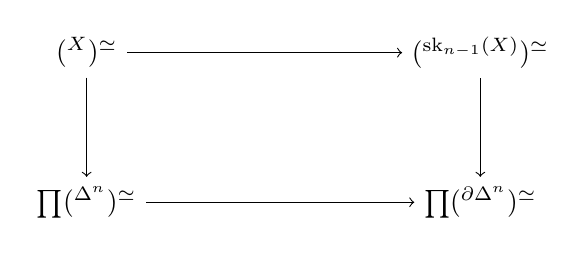
\begin{tikzpicture}
  \node (tl) at (0,0) {$(\C^X)^{\simeq}$};
  \node (tr) at (5.0,0) {$(\C^{\mathrm{sk}_{n-1}(X)})^{\simeq}$};
  \node (bl) at (0,-1.9) {$\prod (\C^{\Delta^n})^{\simeq}$};
  \node (br) at (5.0,-1.9) {$\prod (\C^{\partial \Delta^n})^{\simeq}$};
  \draw[->] (tl) -- (tr);
  \draw[->] (tl) -- (bl);
  \draw[->] (tr) -- (br);
  \draw[->] (bl) -- (br);
\end{tikzpicture}
\end{center}
其中下面的水平映射是\trKanFibration{}的一个乘积，从而自身是一个%
\trKanFibration{}。我们由\cref{lem:pullback-weak-equivalence} 结束这一情形。

为了证明一般的情形，我们现在把任意\trSimplicialSet{} $X$ 写成其骨架之上的
$\N$-指标\trColimit{}。于是我们得到一个同构
\[
(\C^X)^{\simeq} \cong \lim_n (\C^{\mathrm{sk}_n(X)})^{\simeq},
\]
而且描写该\trInverseLimit{}的图表中的所有过渡映射都是\trKanFibration{}（因为
它们是沿\trMonomorphism{}的限制）。我们用\cref{lem:inverse-limit-weak-equivalence}
得出断言。
\end{proof}
